\chapter{Results}
\label{ch:results}
\section{Quantization error minimization training}
Our quantization error minimization training on AlexNet achieves $54\%$ accuracy with the following setting in \autoref{tab:alex_train}. Note that we apply quantization on the first layer as well, and some of the model shape doesn't follow a typical AlexNet model. The input bit-length stays 8-bit as original. \autoref{tab:acc_comp} shows the classification accuracy of several works on ImageNet using AlexNet, note that the first layer of XNOR-net is not quantized, and possibly pose a large computational overhead over quantized one. 
\begin{table}[h]
    \caption{AlexNet 4-bit quantization}
    \label{tab:alex_train}
    \centering
    \footnotesize 
        \begin{tabular}{c|cccccccc}
        \toprule
        layer & conv1 & conv2 & conv3 & conv4 & conv5 & Fc1 & Fc2 & Fc3\\
        \midrule
        Weight & 4 & 4 & 4 & 4 & 4 & 2 & 2 & 32 \\
        Activation & 4 & 4 & 4 & 4 & 4 & 4 & 4 &32\\
        Output channels & 64 & 256 & 256 & 256 & 256 & 4096 & 4096 & 1000\\
        \bottomrule
        \end{tabular}
\end{table}
\begin{table}[h]
    \caption{Classification Accuracy on ImageNet, AlexNet}
    \label{tab:acc_comp}
    \centering
    \footnotesize 
        \begin{tabular}{c|c|c|c|}
        \toprule
        &XNOR-Net\cite{XnorNet} & TensorRT\cite{TensorRT8bit} & OUR\\ 
        \midrule
        Bit-length & 1& 8 & 4 \\
        Accuracy & 44.2\% & 57\% & 54\%\\
        \bottomrule
        \end{tabular}
\end{table}
\section{Implementation results}
We synthesize and evaluate our design using TSMC 90nm technology. The PE array and Buffer specification is provided in \autoref{tab:spec}, the best synthesized cell area is 15698896 cell area, approximately 15.6 $mm^2$. We co-simulate the design using \textbf{Nicotb}\cite{nicotb} and Cadence nc-verilog version 15.20-s039; we synthesize the design with Synopsys design compiler version 0-2018.06 and finally simulate power consumption with Synopsys PrimeTime version M-2017.06-SP2. \autoref{tab:comp} lists several highly related hardware implementation works in comparison, note that Vgg16 benchmark setting is not yet trained on 4-bit arithmetic setting, yet we are highly confident that there is room for quantization for such redundant network. \\
\begin{table}[h]
    \caption{System specification}
    \label{tab:spec}
    \centering
    \footnotesize 
        \begin{tabular}{c|c}
        \toprule
        \midrule
        Technology & TSMC 90nm GUTM Arm f1.0\\
        Gate count (logic only) & 1340.7k (NAND2)\\
        Area & 15.6$mm^2$\\
        PE dimension & 16x16\\
        On-chip SRAM & 124KB\\
        Register file & 56K+384B\\
        Clock rate & 200-400MHz\\
        Peak throughput & 51.2N-102.4N GOPs, N=16,8,4,2\\
        Arithmetic precision & re-configurable 1,2,4,8-bit fixed-point\\
        Average full power & 672mW @200MHz\\
        Power efficiency & 76.19N-152.38N GOPs/W, N=16,8,4,2\\
        \bottomrule
        \end{tabular}
\end{table}
\begin{table}[h]
    \caption{System specification comparison.}
    \label{tab:comp}
    \centering
    \footnotesize 
        \resizebox{\linewidth}{!}{%
        \begin{tabular}{c|cccc}
        \toprule
        Work & JSSC'17\cite{Eyeriss}  & VLSI'16\cite{PrecisionScalableVLSI} & ISSCC'17\cite{ENVISION}   & This work N=16,8,4,2\\
        \midrule
        Technology & 65nm LP CMOS & 40 LP CMOS & 28nm UTBB FD-SOI & 90nm CMOS\\
        Tape-out  & V & V & V & pre-sim\\
        \midrule
        Frequency & 200 & 200 & 200 & 400\\
        Supply voltage  & 1 & 1.1 & 1 & 1\\
        Peak GOPs& 67 & 102 & nx102 n=1,2,4 & Nx152.38 \\
        \midrule
        Area $(mm^2)$ & 12.25 & 2.4 & 1.87 & 15.6\\
        \# of MACs & 168 & 256 & nx256 n=1,2,4 & Nx256\\
        Gate Counts & 1.176M &  1.6M & 1.95M & 1.34M\\
        On-chip memory (KB) & 184.5 & 144 & 144 & 180\\
        \midrule
        Precision & 16-bit fixed & Dynamic 1-16 & Dynamic n x 1-16/n & 1,2,4,8\\
        \midrule
        AlexNet benchmark & 278mW @34.7fps &  76mW @ 47fps & 44mW @47fps & 506mW avg @206.9fps,4b\\
        Vgg16 benchmark   & 236mW @0.7fps  & -             & 26mW @1.67fps & 586mW @ 6.86fps,4b,N/A acc\\
        
        \bottomrule
        \end{tabular} }
\end{table}

\subsection{Area and power}
\autoref{fig:area_breakdown} shows the area breakdown chart for this work, PE logic takes up 25\% of area in contrast to $75\%$ of memory, which actually accounts for a large portion in comparison to related work, as multipliers in \cite{Eyeriss} takes up $7.4\%$ of area. 
\begin{figure}[h]
    \centering
    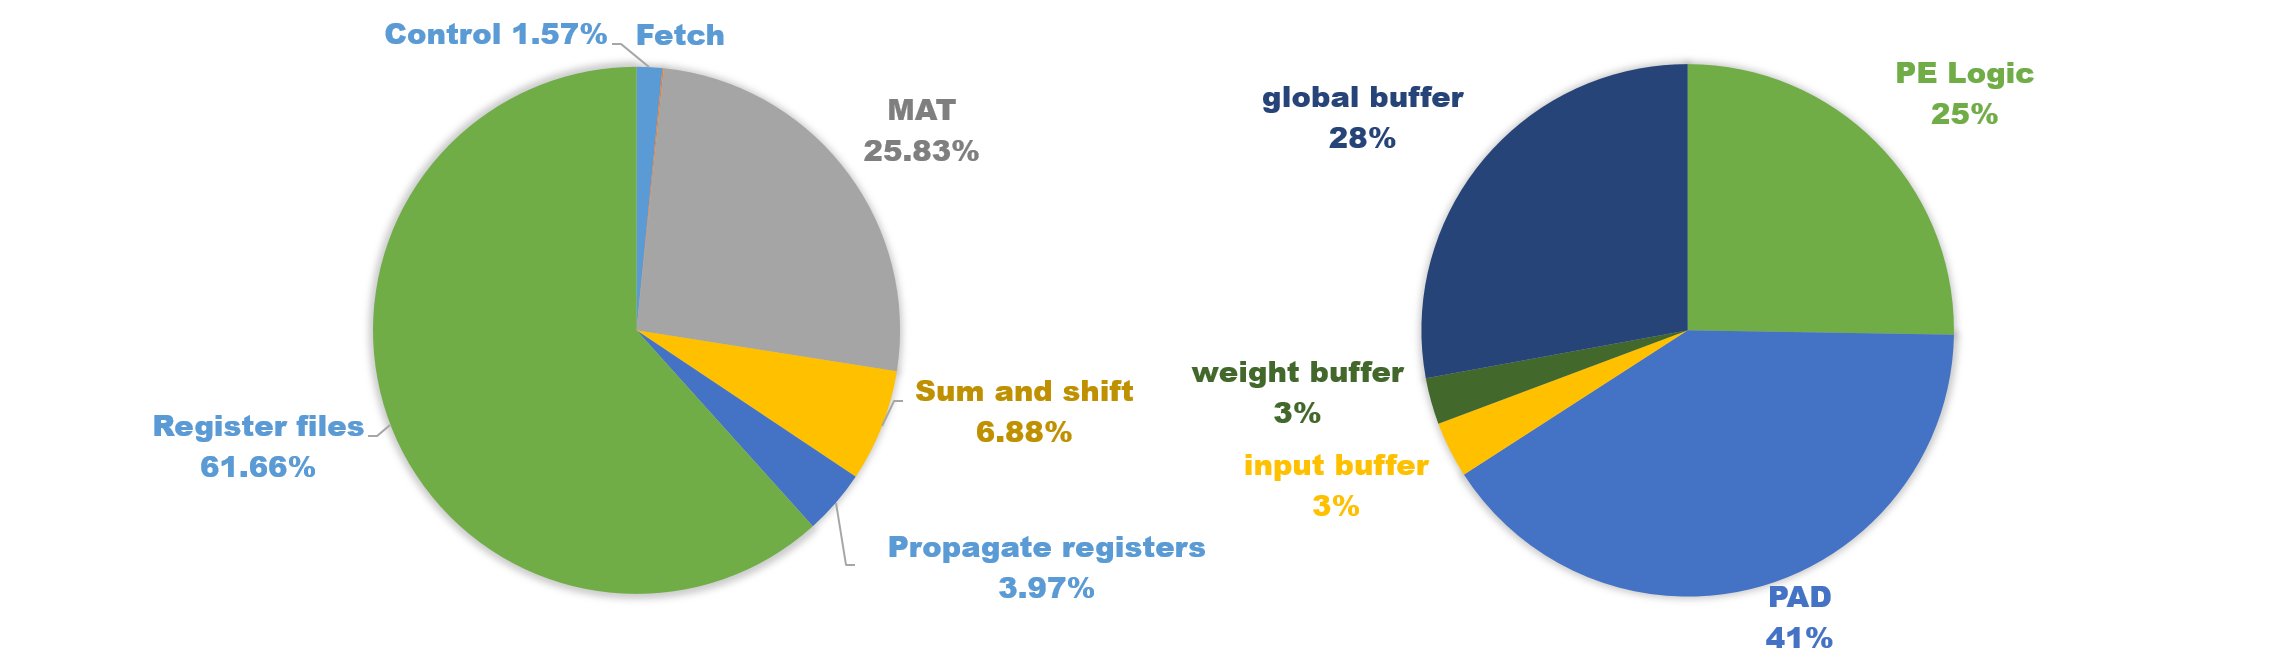
\includegraphics[width=1\linewidth]{inc/5_results/figure/area_breakdown.png}
    \caption{Area breakdown of the system.}
    \label{fig:area_breakdown}
\end{figure}
\begin{table}[h]
    \caption{PE column area gate counts}
    \label{tab:area_gate}
    \centering
    \footnotesize 
        \begin{tabular}{clccccccc}
        \toprule
        control  & Fetch  & MAT       & Sum and shift       & Propagator      & IPAD     & PPAD     & WPAD    & total       \\
        \midrule
        3670 & 200 & 60503 & 16122 & 9295 & 2756 & 74856 & 66802 & 234207\\
        \bottomrule
        \end{tabular}
\end{table}
\autoref{fig:buffer_hier} shows the buffer hierarchy significance, removing input and weight buffer introduces a $1.14$x power consumption overhead on representative AlexNet conv5 layer. The additional buffer takes up about $20\%$ more area as a trade-off. 
\begin{figure}[h]
    \centering
    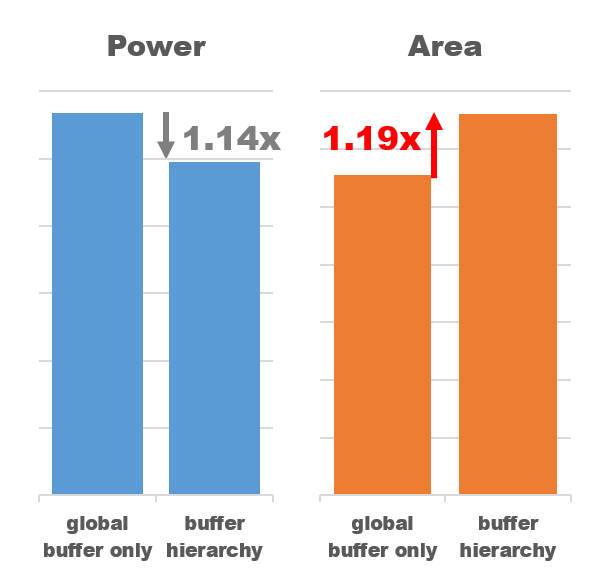
\includegraphics[width=0.6\linewidth]{inc/5_results/figure/buffer_hier.png}
    \caption{Buffer hierarchy area power trade-off.}
    \label{fig:buffer_hier}
\end{figure}
\autoref{fig:power_breakdown} shows the power breakdown of the system. The PE array consumes most portion of the power, indicating workloads falls mainly on the most power efficient part of the system. The PAD access, MAT, sum and shift draws close amount of power. \autoref{tab:power} shows a 4-bit layer power consumption simulated at 200MHz, 1V. \autoref{fig:operation_power} shows the power consumption of different bit mode setting on MAT, indicating that the low-precision operations contributes mainly on memory access saving, the system benefits from arithmetic operation lightly.
\begin{figure}[h]
    \centering
    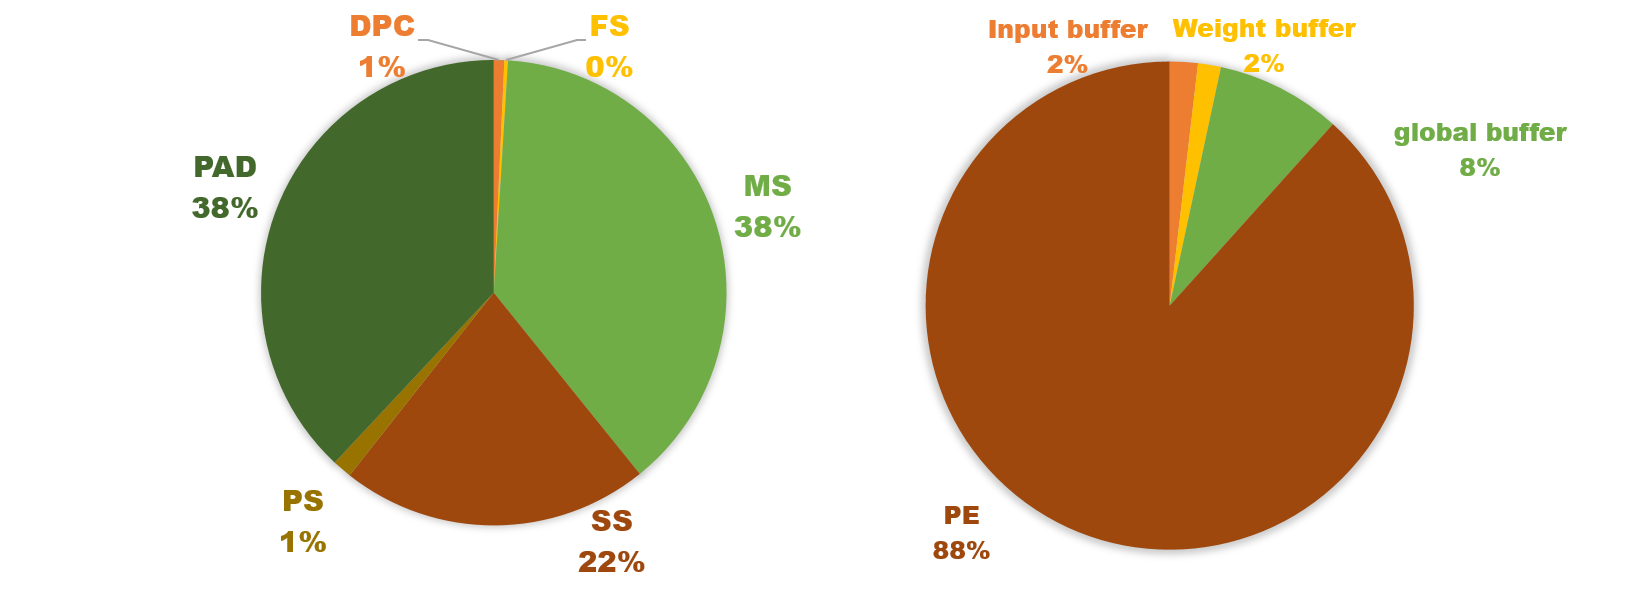
\includegraphics[width=1\linewidth]{inc/5_results/figure/power_breakdown.png}
    \caption{Average power breakdown of the system.}
    \label{fig:power_breakdown}
\end{figure}

\begin{figure}
    \centering
    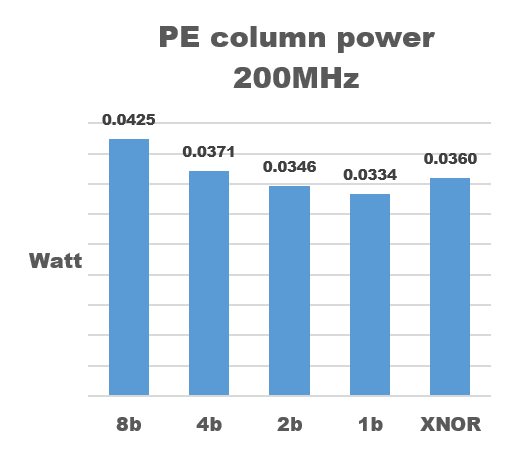
\includegraphics[width=0.6\linewidth]{inc/5_results/figure/operation_power.png}
    \caption{Arithmetic unit configuration power.}
    \label{fig:operation_power}
\end{figure}
\begin{table}[h]
    \caption{System average power (mW) consumption at 200MHz}
    \label{tab:power}
    \centering
    \footnotesize 
        \begin{tabular}{cccccccc}
        DPC  & FS   & MS    & SS     & PS   & PAD     & buffer hierarchy & total   \\
        \toprule
        4.16 & 1.44 & 219 & 122. & 7.68 & 218 & 79.1           & 652.5\\
        \bottomrule
        \end{tabular}
\end{table}





\begin{table}[h!]
    \caption{Performance summary Batch=4}
    \label{tab:perf_sum}
    \centering
    \footnotesize 
    \resizebox{\linewidth}{!}{%
        \begin{tabular}{c|ccccc}
                      & FPS & processing time (s)& off-chip access(MB) & average power (mW) & Accuracy(\%)   \\
        \toprule
        AlexNet       & 206.9  & 0.019 & 5.84   & 573   &  54               \\
        Vgg16         & 6.86   & 0.58  & 210.01 & 664   & N/A              \\
        Alex XNOR     & 491.2  & 0.008 & 2.99   & 581   & 44 \\
        TensorRT Alex 8-bit    & 116.5    & 0.034 & 13.95  & 580   & 57   \\
        \bottomrule
        \end{tabular}
    }
\end{table}
\subsection{Experiments} 
We lists the configuration and setting used on various models, and the performance reports. All the experiments set the batch size $B$ to 4, processes at 200MHz, 1V. Note the $psum\ word$ parameter is the partial sum word length storage on-chip, a word is of 16-bit, we use 2 word 32-bit for partial sum when overflow takes place frequently. Our hardware utilization rate is easily determined, which is usually $T_h$, the active PE column counts as well as the output rows processed in a PE row. If $T_h$ is larger than the PE column number 16, we allocate as much resource, as in PE columns as possible, and gated idle PE columns at the last height tile. For the most part, our hardware utilization rate on ImageNet, where the input spatial size is of 224x224, is usually $13/16(81.25\%)$. The utilization rate can be easily scaled up if we fit the design to a particular dataset spatial dimension, however we choose the PE shape for general purpose, and multiple of 16 is usually suitable for hardware designs. From various experiments we can see the power of quantization as low as to 4-bit, it boosts the processing time and reduce off-chip memory access even without coding or compression at the edge of the system. More importantly, the design is highly flexible and fit for various bit-length and model shapes. \\

\begin{table}[h!]
    \caption{AlexNet configurations}
    \label{tab:alex_conf}
    \centering
    \footnotesize 
    \resizebox{\linewidth}{!}{%
        \begin{tabular}{l|lllllllllllllllllll}
                      & $T_w$ & $T_h$ & $H'$ & $W'$ & $P_{ch}$ & $X_b$ & $W_b$ & $A_b$ & $O_b$ & $P_m$ & $R$  & $S$  & $T_m$ & $T_b$ & $C$   & $E$  & $F$  & $M$   & psum word \\
                      \toprule
        alex conv1     & 14 & 14 & 63 & 63 & 1   & 2  & 1  & 4  & 4  & 2  & 11 & 11 & 64 & 2  & 3   & 55 & 55 & 64  & 2         \\
        alex conv2     & 27 & 27 & 31 & 31 & 2   & 1  & 1  & 4  & 4  & 2  & 5  & 5  & 64 & 1  & 64  & 27 & 27 & 256 & 1         \\
        alex conv3,4,5     & 13 & 13 & 15 & 15 & 4   & 1  & 1  & 4  & 4  & 4  & 3  & 3  & 64 & 4  & 256 & 13 & 13 & 256 & 1         \\
        old alex conv3 & 13 & 13 & 15 & 15 & 4   & 1  & 1  & 4  & 4  & 4  & 3  & 3  & 64 & 4  & 256 & 13 & 13 & 384 & 1         \\
        old alex conv4 & 13 & 13 & 15 & 15 & 4   & 1  & 1  & 4  & 4  & 4  & 3  & 3  & 64 & 4  & 192 & 13 & 13 & 384 & 1         \\
        old alex conv5 & 13 & 13 & 15 & 15 & 4   & 1  & 1  & 4  & 4  & 4  & 3  & 3  & 64 & 4  & 192 & 13 & 13 & 256 & 1         \\

        \bottomrule
        \end{tabular}
    }
\end{table}
\begin{table}[h!]
    \caption{Vgg-16 configurations}
    \label{tab:vgg_conf}
    \centering
    \footnotesize 
    \resizebox{\linewidth}{!}{%
        \begin{tabular}{l|llllllllllllllllllllll}
                & $T_w$ & $T_h$ & $H'$ & $W'$ & $P_{ch}$ & $X_b$ & $W_b$ & $A_b$ & $O_b$ & $P_m$ & $R$  & $S$  & $T_m$ & $T_b$ & $C$   & $E$  & $F$  & $M$   & psum word \\
        \toprule
            vgg1   & 16 & 16 & 18 & 18 & 4   & 2  & 1  & 4  & 4  & 2  & 3 & 3 & 64 & 2  & 3   & 224 & 224 & 64  & 2         \\
            vgg1-2 & 16 & 16 & 18 & 18 & 4   & 1  & 1  & 4  & 4  & 4  & 3 & 3 & 64 & 4  & 64  & 224 & 224 & 64  & 1         \\
            vgg2-1 & 16 & 16 & 18 & 18 & 4   & 1  & 1  & 4  & 4  & 4  & 3 & 3 & 64 & 4  & 64  & 224 & 224 & 128 & 1         \\
            vgg2-2 & 16 & 16 & 18 & 18 & 4   & 1  & 1  & 4  & 4  & 4  & 3 & 3 & 64 & 4  & 128 & 112 & 112 & 128 & 1         \\
            vgg3-1 & 16 & 16 & 18 & 18 & 4   & 1  & 1  & 4  & 4  & 4  & 3 & 3 & 64 & 4  & 128 & 112 & 112 & 256 & 1         \\
            vgg3-2,3 & 16 & 16 & 18 & 18 & 4   & 1  & 1  & 4  & 4  & 4  & 3 & 3 & 64 & 4  & 256 & 56  & 56  & 256 & 1         \\
            vgg4-1 & 16 & 16 & 18 & 18 & 4   & 1  & 1  & 4  & 4  & 4  & 3 & 3 & 64 & 4  & 256 & 56  & 56  & 512 & 1         \\
            vgg4-2,3 & 16 & 16 & 18 & 18 & 4   & 1  & 1  & 4  & 4  & 4  & 3 & 3 & 64 & 4  & 512 & 28  & 28  & 512 & 1         \\
            vgg5-1 & 15 & 15 & 18 & 18 & 4   & 1  & 1  & 4  & 4  & 4  & 3 & 3 & 64 & 4  & 512 & 28  & 28  & 512 & 1         \\
            vgg5-2,3 & 14 & 14 & 18 & 18 & 4   & 1  & 1  & 4  & 4  & 4  & 3 & 3 & 64 & 4  & 512 & 14  & 14  & 512 & 1         \\

        \bottomrule
        \end{tabular}
    }
\end{table}

\begin{table}[h!]
    \caption{XNOR AlexNet configurations}
    \label{tab:alex_conf}
    \centering
    \footnotesize 
    \resizebox{\linewidth}{!}{%
        \begin{tabular}{l|lllllllllllllllllll}
                      & $T_w$ & $T_h$ & $H'$ & $W'$ & $P_{ch}$ & $X_b$ & $W_b$ & $A_b$ & $O_b$ & $P_m$ & $R$  & $S$  & $T_m$ & $T_b$ & $C$   & $E$  & $F$  & $M$   & psum word \\
                      \toprule
            alexnor conv1     & 14 & 14 & 63 & 63 & 1   & 1  & 1  & 8  & 1  & 2  & 11 & 11 & 64 & 2  & 3   & 55 & 55 & 64  & 2         \\
            alexnor conv2     & 27 & 27 & 31 & 31 & 2   & 1  & 1  & 1  & 1  & 2  & 5  & 5  & 64 & 1  & 64  & 27 & 27 & 256 & 1         \\
            alexnor conv3 & 13 & 13 & 15 & 15 & 4   & 1  & 1  & 1  & 1  & 4  & 3  & 3  & 96 & 4  & 256 & 13 & 13 & 384 & 1         \\
            alexnor conv4 & 13 & 13 & 15 & 15 & 4   & 1  & 1  & 1  & 1  & 4  & 3  & 3  & 96 & 4  & 192 & 13 & 13 & 384 & 1         \\
            alexnor conv5 & 13 & 13 & 15 & 15 & 4   & 1  & 1  & 1  & 1  & 4  & 3  & 3  & 96 & 4  & 192 & 13 & 13 & 256 & 1       \\

        \bottomrule
        \end{tabular}
    }
\end{table}

\begin{table}[h!]
    \caption{TensorRT 8-bit AlexNet configurations}
    \label{tab:alex8b_conf}
    \centering
    \footnotesize 
    \resizebox{\linewidth}{!}{%
        \begin{tabular}{l|lllllllllllllllllll}
                      & $T_w$ & $T_h$ & $H'$ & $W'$ & $P_{ch}$ & $X_b$ & $W_b$ & $A_b$ & $O_b$ & $P_m$ & $R$  & $S$  & $T_m$ & $T_b$ & $C$   & $E$  & $F$  & $M$   & psum word \\
                      \toprule
            alex 8b conv1     & 14 & 14 & 63 & 63 & 1   & 1  & 1  & 8  & 8  & 2  & 11 & 11 & 64 & 2  & 3   & 55 & 55 & 64  & 2         \\
            alex 8b conv2     & 27 & 14 & 31 & 31 & 2   & 1  & 1  & 8  & 8  & 1  & 5  & 5  & 64 & 1  & 64  & 27 & 27 & 256 & 2         \\
            alex 8b conv3     & 13 & 13 & 15 & 15 & 4   & 1  & 1  & 8  & 8  & 2  & 3  & 3  & 64 & 4  & 256 & 13 & 13 & 384 & 2         \\
            alex 8b conv4     & 13 & 13 & 15 & 15 & 4   & 1  & 1  & 8  & 8  & 2  & 3  & 3  & 64 & 4  & 192 & 13 & 13 & 384 & 2         \\
            alex 8b conv5     & 13 & 13 & 15 & 15 & 4   & 1  & 1  & 8  & 8  & 2  & 3  & 3  & 64 & 4  & 192 & 13 & 13 & 256 & 2       \\

        \bottomrule
        \end{tabular}
    }
\end{table}

\begin{table}[h!]
    \caption{AlexNet results}
    \label{tab:alex_result}
    \centering
    \footnotesize 
    \resizebox{\linewidth}{!}{%
        \begin{tabular}{l|llllll}
                      & ibuf size (B) & wbuf size (B) & psum pad (2B) & gb size (B) & off-chip access (MB) & prcessing time (ms) \\
        \toprule
        alex conv1     & 1008          & 484           & 56                & 97416       & 1.82                 & 4.34                \\
        alex conv2     & 248           & 200           & 54                & 56900       & 1.61                 & 6.91                \\
        alex conv3,4,5     & 120           & 288           & 52                & 55072       & 0.80                 & 2.40                \\
        old alex conv5 & 120           & 288           & 52                & 55072       & 0.62                 & 1.80                \\
        old alex conv4 & 120           & 288           & 52                & 55072       & 0.93                 & 2.70                \\
        old alex conv3 & 120           & 288           & 52                & 55072       & 1.20                 & 3.59                \\
        \midrule
          total(ours/typical)    &               &               &                   &             & 5.84/6.19                    & 18.44/19.34         \\

        \bottomrule
        \end{tabular}
    }
\end{table}
\begin{table}[h!]
    \caption{Vgg results}
    \label{tab:vgg_result}
    \centering
    \footnotesize 
    \resizebox{\linewidth}{!}{%
        \begin{tabular}{l|llllll}
               & ibuf size (B) & wbuf size (B) & psum pad (2B) & gb size (B) & off-chip access (MB) & prcessing time (ms) \\
        \toprule
        vgg1   & 288           & 288           & 64               & 80512       & 11.72                & 18.06               \\
        vgg1-2 & 144           & 288           & 64                & 80512       & 17.32                & 36.13               \\
        vgg2-1 & 144           & 288           & 64                & 80512       & 25.46                & 72.25               \\
        vgg2-2 & 144           & 288           & 64                & 80512       & 14.26                & 36.13               \\
        vgg3-1 & 144           & 288           & 64                & 80512       & 23.93                & 72.25               \\
        vgg3-2 & 144           & 288           & 64                & 80512       & 16.63                & 47.19               \\
        vgg3-3 & 144           & 288           & 64                & 80512       & 16.63                & 47.19               \\
        vgg4-1 & 144           & 288           & 64                & 80512       & 30.25                & 94.37               \\
        vgg4-2 & 144           & 288           & 64                & 80512       & 15.63                & 47.19               \\
        vgg4-3 & 144           & 288           & 64                & 80512       & 15.63                & 47.19               \\
        vgg5-1 & 144           & 288           & 60                & 72576       & 14.88                & 44.24               \\
        vgg5-2 & 144           & 288           & 56                & 65152       & 3.85                 & 10.32               \\
        vgg5-3 & 144           & 288           & 56                & 65152       & 3.85                 & 10.32               \\
        \midrule
           total    &               &               &                   &             & 210.01               & 582.82             \\

        \bottomrule
        \end{tabular}
    }
\end{table}

\begin{table}[h!]
    \caption{Xnor AlexNet results}
    \label{tab:xnor_result}
    \centering
    \footnotesize 
    \resizebox{\linewidth}{!}{%
        \begin{tabular}{l|llllll}
                      & ibuf size (B) & wbuf size (B) & psum pad (2B) & gb size (B) & off-chip access (MB) & prcessing time (ms) \\
        \toprule
        alexnor conv1 & 504           & 484           & 56                & 81540       & 2.01                 & 4.34                \\
        alexnor conv2 & 248           & 200           & 54                & 56900       & 0.40                 & 1.73                \\
        alexnor conv3 & 120           & 288           & 52                & 79008       & 0.25                 & 0.90                \\
        alexnor conv4 & 120           & 288           & 52                & 79008       & 0.19                 & 0.67                \\
        alexnor conv5 & 120           & 288           & 52                & 79008       & 0.14                 & 0.51                \\
        \midrule
            total          &               &               &                   &             & 2.99                 & 8.14                \\

        \bottomrule
        \end{tabular}
    }
\end{table}

\begin{table}[h!]
    \caption{TensorRT AlexNet results}
    \label{tab:xnor_result}
    \centering
    \footnotesize 
    \resizebox{\linewidth}{!}{%
        \begin{tabular}{l|llllll}
                      & ibuf size (B) & wbuf size (B) & psum pad size (B) & gb size (B) & off-chip access (MB) & prcessing time (ms) \\
        \toprule
        alexnet 8b conv1 & 504           & 484           & 56                & 81540       & 2.68                 & 4.34                \\
        alexnet 8b conv2 & 248           & 100           & 54                & 58628      & 5.74                 & 13.82               \\
        alexnet 8b conv3 & 120           & 288           & 52                & 98336       & 2.41                 & 7.19                \\
        alexnet 8b conv4 & 120           & 288           & 52                & 98336       & 1.87                 & 5.39                \\
        alexnet 8b conv5 & 120           & 288           & 52                & 98336       & 1.25                 & 3.59                \\
        \midrule
                total      &               &               &                   &             & 13.95               & 34.33   \\
        \bottomrule
        \end{tabular}
    }
\end{table}



\autoref{fig:bit_conf} studies the re-configurablility benefits and trade-offs on various bit-length setting. Most interesting part is the mixed precision flexibility of this work, as long as the training results permits, the potential presents. The figure compares the off-chip memory access and processing cycle counts on our AlexNet conv5 setting. As the data bit-length varies, the optimal arithmetic mode can be chosen based on the charts. Possibilities exist where the cost is close for two arithmetic configuration, the better choice lies in the trade-off between saving off-chip DRAM power consumption which is often 3-orders higher than a basic operation and saving processing cycle on a averagely 600mW system.

\begin{figure}[hbt!]
    \centering
    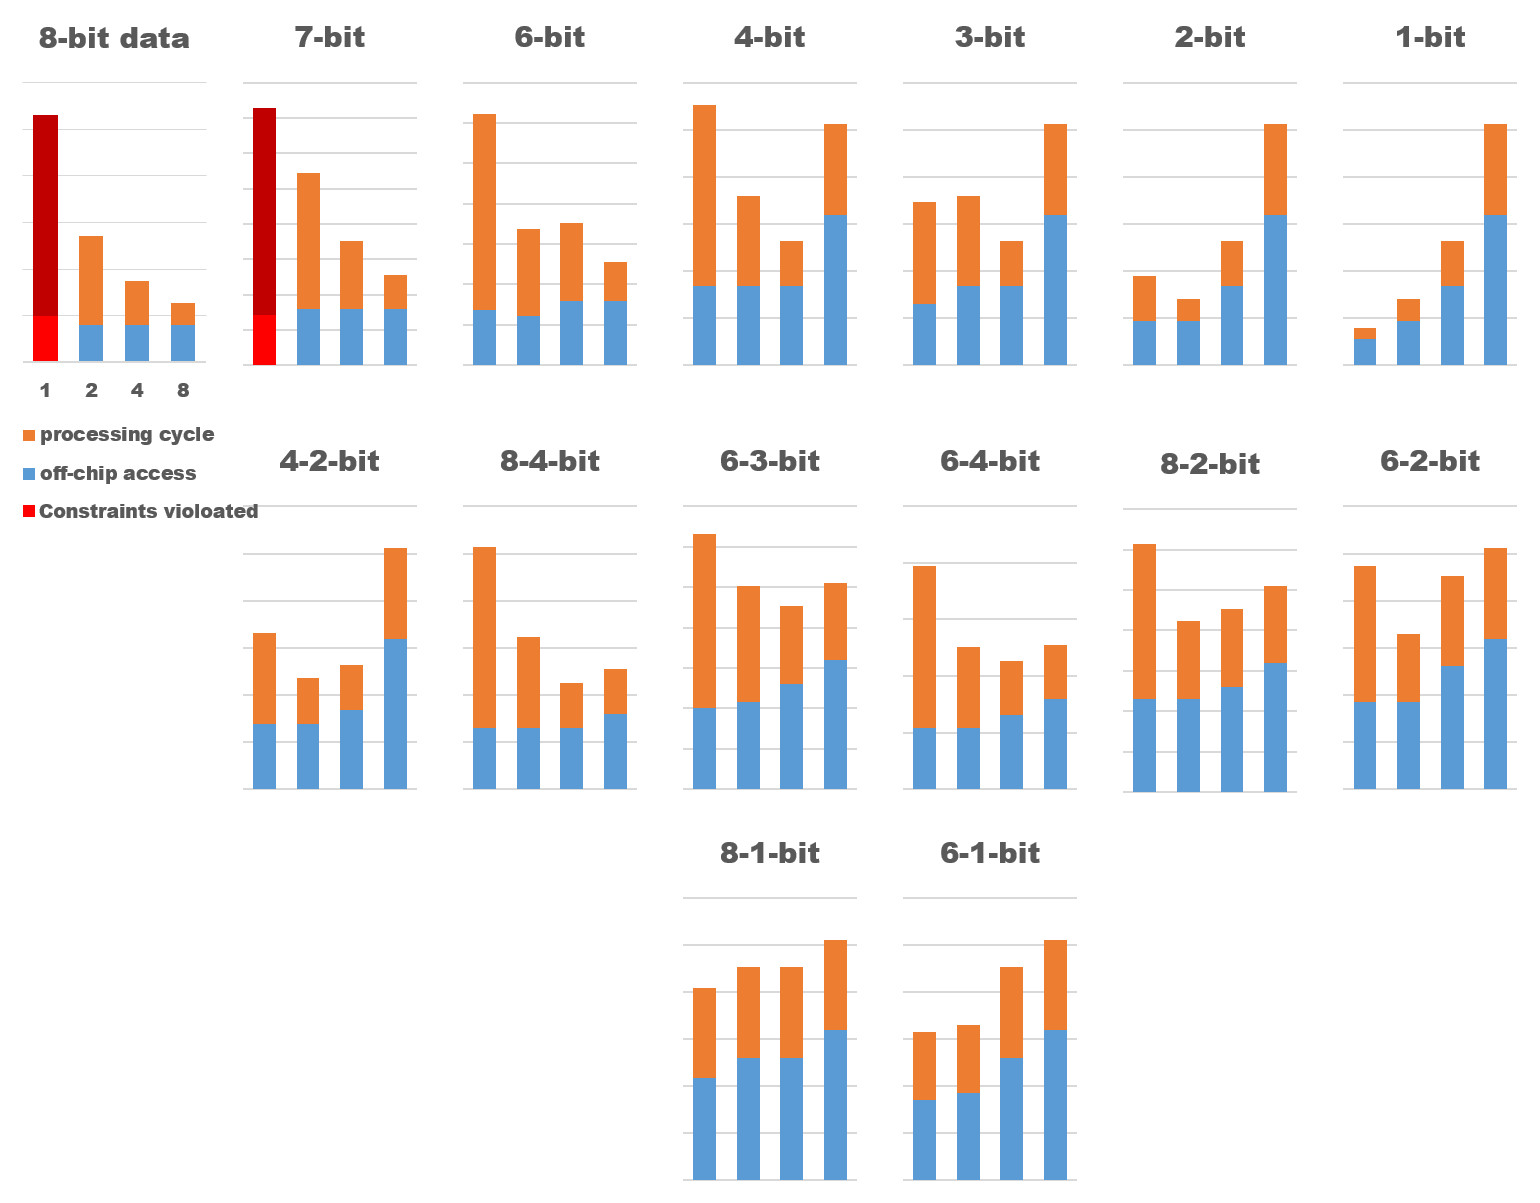
\includegraphics[width=1\linewidth]{inc/5_results/figure/bit_conf.png}
    \caption{Various data bit-length to arithmetic bit-length off-chip access and processing time scaling.}
    \label{fig:bit_conf}
\end{figure}

